\documentclass{article}

% Language setting
% Replace `english' with e.g. `spanish' to change the document language
\usepackage[english,main=spanish]{babel}

% Set page size and margins
% Replace `letterpaper' with `a4paper' for UK/EU standard size
\usepackage[letterpaper,top=2cm,bottom=2cm,left=3cm,right=3cm,marginparwidth=1.75cm]{geometry}

% Useful packages
\usepackage{hyperref}
\hypersetup{linktoc=all}
\usepackage[utf8]{inputenc}
\usepackage[T1]{fontenc}
%%Fuente, probar otras
\usepackage{palatino}
%%Otros paquetes
\usepackage{graphicx}
\usepackage[table,xcdraw]{xcolor}
\usepackage{physics}
\usepackage{amssymb}
\usepackage{amsmath}
\usepackage{caption}
\usepackage{float}
\usepackage{listingsutf8}
\usepackage{csquotes}
\usepackage{ragged2e}
\usepackage{flafter}
\usepackage{listings}             
%References in toc
\usepackage[nottoc]{tocbibind}
% Citas
\usepackage[sorting=none,style=phys]{biblatex}
\addbibresource{sample.bib}

\title{Nanofoams Creator}
\author{Nicolás Vazquez, Carlos Ruestes, Emmanuel Millán}

\begin{document}
\maketitle
\tableofcontents

\section{Introducción}

Esta herramienta fue creada en el marco de una investigación que se dedicó al estudio de las propiedades mecánicas de los metales nanoporosos de tipo bcc. A saber nuestro, no se contaba hasta el momento con una herramienta que pudiera generar estas estructuras para las simulaciones de dinámica molecular. La misma se basa en una implementación de un trabajo previo de Soyarslan et al. \cite{Soyarslan2018}. 

Esta herramienta fue programada en Python, y tiene dos versiones, que en esencia hacen lo mismo pero están implementadas sobre diferente hardware: 

\begin{itemize}
    \item La primera versión corre por línea de comandos, mediante ejecución del script \verb+build_nanofoams.py+, que requiere además un cierto script de entrada, cuyo template es el archivo \verb+nanofoams_input.txt+
    \item La segunda versión está implementada dentro del framework TensorFlow, y está pensada para su uso con aceleración por GPU. La presentación fue hecha en formato Jupyter Notebook, y se puede utilizar dentro de la plataforma de cómputo en la nube Google Colab. 
\end{itemize}

Sin más preámbulo, en las siguientes páginas comentaremos brevemente el fundamento teórico detrás del algoritmo, y también se añaden algunas pruebas de rendimiento que se realizaron en el marco de la validación de la herramienta. 

\section{Fundamento teórico} \label{cap:Generacion_muestras}

Los metales nanoporosos son un caso particular de un tipo de microestructura tipo \textit{estocástica bicontinua}. Estas estructuras presentan dos fases contiguas interpenetradas, y son características de muchos materiales. Algunos ejemplos se encuentran en las aleaciones producidas mediante descomposición espinodal, o los metales nanoporosos producidos por corrosión selectiva \cite{Weissmuller2009}. 

En este contexto, la generación de modelos computacionales fidedignos resulta clave para la correcta evaluación de estos materiales. El esquema tradicional de preparación de muestras nanoporosas se ha basado principalmente en el método de campo de fase \textit{(phase-field)} mediante la ecuación de Cahn-Hilliard \cite{CROWSON2007,Farkas2013}, y métodos Monte Carlo \cite{Ngo2015}. Usualmente, una dificultad en esta tarea es el costo computacional de preparar la topología requerida en las muestras, especialmente para sistemas de gran tamaño, factor que ha dificultado el avance de las investigaciones. 

Recientemente, un trabajo de Soyarslan et al. \cite{Soyarslan2018}, propone un nuevo método para la generación de estructuras bicontinuas periódicas, basado en la superposición de ondas sinusoidales con longitud de onda fija y un conjunto fijo de direcciones, en una celda cúbica. Este método ha sido aplicado exitosamente en la generación de muestras para simulaciones mediante elementos finitos \cite{Soyarslan2018} y MD \cite{Liu2019}. Para la generación de las espumas nanoporosas sobre las que se realizaron posteriormente los ensayos de tracción-compresión, se escribió un código inspirado en este método, para la generación de estructuras bicontinuas de forma sencilla y eficiente.

Posteriormente, una segunda etapa fundamental en este proceso de generación de muestras representativas es el diseño de un esquema de relajación y minimización de la muestra previo a los ensayos de deformación. Este contenido se desarrollará a lo largo del siguiente capítulo.

\subsection{El modelo de Soyarslan}
A continuación se presenta un breve resumen adaptado del modelo teórico detrás del código con el que se generaron las espumas nanoporosas\footnote{Para más detalles, el lector puede referirse al artículo original \cite{Soyarslan2018}.}.

Un \textit{elemento de volumen representativo} $\mathcal{V}\subset \mathbb{R}^3$ es una porción de material, que en virtud de sus dimensiones características, es capaz de reproducir de manera fidedigna una o varias de sus características macroscópicas de interés, de ese mismo material. En nuestras estructuras, este volumen está compuesto por dos fases: la fase sólida metálica, y la fase porosa, cuyos volúmenes son respectivamente $\mathcal{B}$ y $\mathcal{P}$. Se tiene entonces, que $\mathcal{V} = \mathcal{B}+\mathcal{P}$. Por último, se denota la interfase de la microestructura por $\partial\mathcal{B}$.

En su artículo de 1965, Cahn mostró que el campo de composición de estas estructuras puede aproximarse como la superposición de infinitas ondas con dirección aleatoria y longitud de onda fija \cite{Cahn1965}. El trabajo de Soyarslan et al. explora una implementación moderna de este campo aleatorio $f$: 

\begin{equation}
    f(\vb{x}) = \sqrt{\frac{2}{N}}\sum_{i=1}^N \cos(\vb{q_i}\vdot\vb{x}+\varphi_i).
    \label{eq:Soyarslan_RandomField}
\end{equation}

En \eqref{eq:Soyarslan_RandomField}, $\vb{x}$ es el vector de posición, $N$ es el número de ondas consideradas en la serie truncada, y $\vb{q_i}$ y $\varphi_i$ denotan la dirección de la onda y la fase de la onda $i$, respectivamente. El número de onda debe ser fijado a un valor constante, es decir $\abs{\vb{q_i}} = q_0$, con direcciones distribuidas de manera uniforma sobre el el ángulo sólido $4\pi$, y fases uniformemente distribuidas entre $0$ y $2\pi$. Bajo estas condiciones, $f(\vb{x})$ es un \textit{campo gaussiano aleatorio}, con $\expval{f}=0$, $\expval{f^2}=1$. La función de correlación de dos puntos viene dada por 
\begin{equation}
    C_2(\vb{x_1,x_2}) = \expval{f(\vb{x_1})f(\vb{x_2})} = \frac{\sin(q_0r)}{q_0r},
    \label{eq:Soyarslan_Corrx1x2}
\end{equation}
donde los brackets indican promedios de ensamble sobre diferentes realizaciones, y $r=\abs{\vb{x_1-x_2}}$. Si $N$ es suficientemente grande\footnote{En este trabajo, $N$ está en el orden de $10^4$, siguiendo las recomendaciones en \cite{Soyarslan2018}.}, el valor de la función $f(\vb{x)}$ para una posición $\vb{x}$ dada sigue una distribución gaussiana: 

\begin{equation}
    P(f) = \frac{1}{\sqrt{2\pi}}e^{-f^2/2},
    \label{eq:Soyarslan_fGauss}
\end{equation}
y la dirección de onda media 
\begin{equation}
    \vb{\nu} = \frac{1}{N} \sum_{i=1}^N \vb{n_i}
\end{equation}
tiende a cero como consecuencia del teorema central del límite. Se sigue de esto que $f$ es una función isotrópica. 

Dada la función aleatoria \eqref{eq:Soyarslan_RandomField}, las diferentes fases del sistema están dadas mediante un valor de corte $\xi$: 

\begin{equation}
\begin{split}
    &\vb{x}\in\mathcal{B}\qquad\text{si}f(\vb{x})<\xi,\\
    &\vb{x}\in\partial\mathcal{B}\;\,\quad\text{si}f(\vb{x})=\xi,\\
    &\vb{x}\in\mathcal{P}\qquad\text{si}f(\vb{x})>\xi.
\end{split}
\label{eq:Soyarslan_CutValuexi}
\end{equation}

Este valor de corte $\xi$ puede correlacionarse con el valor de fracción sólida, definido como $\phi_\mathcal{B}:=\abs{\mathcal{B}}/\abs{\mathcal{V}}$, gracias a las propiedades del campo gaussiano aleatorio: 

\begin{equation}
    \xi(\phi_\mathcal{B}) = \sqrt{2}\operatorname{erf}^{-1}(2\phi_\mathcal{B}-1),
    \label{eq:Soyarslan_xiPhi_b}
\end{equation}
donde $\operatorname{erf}^{-1}(x)$ denota la función error inversa. 

\subsection{Generación de estructuras periódicas}
Las estructuras generadas mediante las ec. \eqref{eq:Soyarslan_RandomField} y \eqref{eq:Soyarslan_CutValuexi} son, en general, no periódicas. La periodicidad puede lograrse seleccionando un número finito de ondas con números de onda enteros en todas las direcciones, y módulo constante. 

A partir de \eqref{eq:Soyarslan_RandomField}, tomamos $\vb{e_1,e_2,e_3}$  como vectores unitarios para formar una base ortonormal en el espacio real, y se pide que los $\vb{q_i}$ tengan la forma 

\begin{equation}
    \vb{q} = \frac{2\pi}{a}(h,k,l),
    \label{eq:Soyarslan_q}
\end{equation}

donde los \textit{índices de Miller} $h,k,l\in\mathbb{Z}$ y $a$ es una constante. De esta forma, se verifica que $f(\vb{x}) = f(\vb{x}+n_1a\vb{e_1}+n_2a\vb{e_2}+n_3a\vb{e_3}),$ con $n_1,n_2$ y $n_3$ enteros arbitrarios. Esto implica que $f$ tiene periodicidad con respecto a los vectores de la base, y con magnitud $a$. Más aún, si en \eqref{eq:Soyarslan_RandomField} se fijan los $\phi_i$ a un valor idéntico, entonces $f$ es también invariante con respecto al intercambio de ejes, y $f$ adquiere la simetría de una red cúbica con parámetro de red $a$. 

De estas consideraciones, se tiene que las estructuras espinodales periódicas pueden ser construidas restringiendo la suma en la ec. \eqref{eq:Soyarslan_RandomField} a un conjunto de $\vb{q_i}$ con un valor dado y constante $H$, tal que
\begin{equation}
H = \sqrt{h^2+k^2+l^2},
\label{eq:H_Soyarslan}
\end{equation}
y donde $\abs{\vb{q}}=q_0=2\pi H/a$. La función $f$ entonces tiene condiciones periódicas en las 3 direcciones, formando celdas unitarias cúbicas e idénticas de lado $a$. 

\subsection{Caracterización morfológica}
El método descrito en \cite{Soyarslan2018}, tiene la ventaja de que a partir de su definición es posible deducir expresiones explícitas para propiedades morfológicas y topológicas de interés, tales como la relación superficie-volumen, el diámetro medio de ligamento, curvatura gaussiana, el genus (una forma de cuantificar la conectividad de la red), etc. Al medir estas cantidades en nuestras espumas generadas, se pudo corroborar el correcto funcionamiento del código implementado, contrastando resultados. A continuación, se dejan listadas algunas de las ecuaciones utilizadas en este trabajo para la caracterización. 

Cada una de las componentes $\cos(\vb{q_i\cdot x})$ que componen el campo gaussiano aleatorio \eqref{eq:Soyarslan_RandomField} tienen una misma longitud de onda $\lambda = 2\pi/q_0$, que puede usarse como una primer estimación de un tamaño característico de la estructura. Sin embargo, un estudio más detallado requiere inspeccionar la función de autocorrelación \eqref{eq:Soyarslan_Corrx1x2}. El primer máximo de esta ecuación está en $q_0 r \approx 1.23 \times 2\pi$, que define una distancia característica $\hat{L}$, entre regiones de máximo valor de $f$. Al ser las espumas estructuras binarias, $\hat{L}$ puede interpretarse como la distancia media entre centros locales de espacio sólido o poroso; más claramente, la distancia promedio entre los centros de dos ligamentos vecinos: 

\begin{equation}
    \hat{L} = 1.23 \frac{2\pi}{q_0}
    \label{eq:Soyarslan_L_hat}
\end{equation}

Otra longitud característica importante de estas espumas nanoporosas es el diámetro medio de ligamento $L$, para la cual el modelo de Soyarslan predice una expresión en función de $\phi_\mathcal{B}$ y de $H$:
\begin{equation}
    L = \frac{a}{H}[0.53\phi_{\mathcal{B}}+0.41],
    \label{eq:Soyarslan_L}
\end{equation}
donde $a$ es la misma constante introducida mediante la ec. \eqref{eq:Soyarslan_q}. En el artículo original, Soyarslan propone esta ecuación tras hacer una ajuste de $L$ en función de $\hat{L}$ y $\phi_B$.

Otra cantidad importante para caracterizar la espuma es la relación entre superficie y volumen o superficie específica $\mathcal{S} = \frac{\abs{\partial\mathcal{B}}}{\abs{\mathcal{V}}}$. La expresión para calcularla es

\begin{equation}
    \mathcal{S} = \frac{2q_0}{\pi\sqrt{3}}e^{-\xi^2/2},
    \label{eq:Soyarslan_S}
\end{equation}
con $\xi$ dependiente de la fracción sólida por la ec. \eqref{eq:Soyarslan_xiPhi_b}.

Por último, para caracterizar la topología de la red, se utiliza el número de genus $G$, que es un parámetro topológico que caracteriza la conectividad de la red \cite{munkres2000topology}. Este número además puede interpretarse como el número de túneles o loops en la estructura; por ejemplo, el genus de una esfera es 0, el de un toroide es 1, y el de un pretzel es 2. Como este valor es una característica extensiva del volumen representativo, lo que suele hacerse es expresarlo de manera reducida por algun tamaño característico, dividiendo por ejemplo por el volumen sólido o total, a veces en conjunto con la relación superficie/volumen \cite{Guillotte2019,Li2019}. En Soyarslan et al. \cite{Soyarslan2018}, se presenta por ejemplo la cantidad $g_V$, que es el $G$ escaleado por el volumen total-volumen sólido más volumen poroso-: 

\begin{equation}
    g_V = \frac{1}{12\pi^2}\frac{q_0^3}{\sqrt{3}}[1-\xi^2]e^{-\xi^2/2}
    \label{eq:Soyarslan_Gv}
\end{equation}

En el artículo de Guillotte et al. \cite{Guillotte2019}, se presenta una densidad de genus reducida $g_v\times \mathcal{S}^{-3}$, que resulta de combinar las expresiones de las ec. \eqref{eq:Soyarslan_S} y \eqref{eq:Soyarslan_Gv}:

\begin{equation}
    g_V \times S^{-3} = \frac{3\pi}{32}[1-\xi^2]e^{\xi^2/2}
    \label{eq:Pizzagalli_g_v}
\end{equation}

Todos estos resultados analíticos son útiles para predecir las características de la espuma previamente a su generación. Por otra parte, si pueden obtenerse por algún otro método estas cantidades, es posible contrastarlos con la teoría para corroborar el correcto funcionamiento del software. Los resultados de este estudio son presentados en la sección \ref{sec:4.1_Software}.

\section{Implementación en código}

En total, se desarrollaron 4 versiones del código, cada una de ellas desarrollando mejoras de manera iterativa: 

\begin{enumerate}
    \item La primera versión fue escrita en lenguaje ``estándar'' de Python, es decir, sin el uso de bibliotecas externas. Esto implica el uso de grandes bucles anidados. Se hicieron algunas mejoras que fueron conservadas en todas las otras versiones, como es por ejemplo el añadido de un pequeño programa capaz de calcular el conjunto de direcciones $[hkl]$ posibles para un valor entero de $H$ dado, para poder generar estructuras periódicas. 
    \item La segunda versión de este código reemplaza el uso de bucles anidados, para redefinir todo en términos de operaciones matriciales. Para ello se hizo uso de la librería de computación científica \textit{NumPy} \cite{Harris2020}. 
    
    En esta nueva implementación (así como en todas las siguientes) se implementó un tensor de rango 3 definido 
    
    \begin{equation}
        T_{ijk} := (\vb{q\vdot x})_{ij} + \phi_k,
    \end{equation}
    para todos los puntos $\vb{x}$ del dominio y para todos los vectores de onda $\vb{q}$ del conjunto de direcciones\footnote{Es decir, para un número $N$ de átomos, un conjunto de $Q$ direcciones y $M$ fases, este tensor tiene dimensiones $N\times Q\times M$}.
    
    Al momento del desarrollo, se vio que la cantidad de memoria necesaria para alojar este tensor en memoria era para todos los casos de interés muy superior al terabyte(Tb), con lo cual se hicieron dos modificaciones importantes, que se conservaron en el resto de las versiones implementadas: 
    \begin{itemize}
        \item Convertir todos los flotantes de doble precisión (estándar para flotante en Python) a flotante de simple precisión. Por sí sola, esta modificación conlleva una reducción del 50\% de costos de memoria. 
        \item Particionar el tensor en subconjuntos para llevar a cabo el cálculo por partes. Para evitar almacenar todo el tensor en memoria de una sola vez, el programa toma un pequeño lote de átomos por vez (del orden de 32) y calcula el tensor, evaluando en ellos la función. 
    \end{itemize}
    Por último, vale la pena mencionar que gracias a ciertas funcionalidades de la creación de grillas en NumPy, el uso de \textit{arrays} permite poder crear dominios con celdas unitarias tipo cúbica, bcc y fcc. Esto también se conservó en versiones posteriores.
    \item La segmentación del tensor en partes más pequeñas e independientes hizo posible repartir el trabajo en los distintos cores del procesador, permitiendo la paralelización del trabajo. Para asignar las distintas tareas a los hilos y procesadores se recurrió al uso de las librerías \textit{joblib} y \textit{loky}\footnote{\url{https://github.com/joblib/loky}}. 
    \item Una vez reescrito el código en términos de operaciones matriciales, se consideró desarrollar una versión alternativa, capaz de utilizar la potencia de cálculo de las GPUs. Esto se pudo llevar a cabo, reescribiendo el código de la versión (2) para funcionar bajo el framework \textit{Tensorflow 2} \cite{tang2016tf}, conocido por su uso extendido en el ámbito del \textit{Machine Learning}. 
\end{enumerate}

Una versión resumida del desarrollo de las distintas versionas del código y las mejoras introducidas está contenido en la tabla \ref{tab:Versiones_nanofoams}.

\begin{table}[h]
\centering
\begin{tabular}{|c|c|l|}
\hline
\textbf{Versión del código} &
  \textbf{Plataforma} &
  \multicolumn{1}{c|}{\textbf{Mejoras introducidas}} \\ \hline
\begin{tabular}[c]{@{}c@{}}1ra\\  (baseline)\end{tabular} &
  \begin{tabular}[c]{@{}c@{}}CPU \\ 1 core/1 thread\end{tabular} &
  \begin{tabular}[c]{@{}l@{}}Versión inicial del código.\\ Esquema de bucles anidados\\ para el cálculo.\end{tabular} \\ \hline
\begin{tabular}[c]{@{}c@{}}2da\\  (NumPy - Single thread)\end{tabular} &
  \begin{tabular}[c]{@{}c@{}}CPU \\ 1core/1 thread\end{tabular} &
  \begin{tabular}[c]{@{}l@{}}Implementación de los cálculos\\ en matrices. Cálculo por batches.\end{tabular} \\ \hline
\begin{tabular}[c]{@{}c@{}}3ra\\  (Numpy - Multi-thread)\end{tabular} &
  \begin{tabular}[c]{@{}c@{}}CPU\\ Multicore/Multi thread\end{tabular} &
  \begin{tabular}[c]{@{}l@{}}Implementación de los cálculos\\ en matrices con división de cálculo\\ por batches en los distintos threads. \\ Optimización para uso en clústers\\ gracias a la paralelización.\end{tabular} \\ \hline
\begin{tabular}[c]{@{}c@{}}4ta \\ (Tensorflow GPU)\end{tabular} &
  GPU &
  \begin{tabular}[c]{@{}l@{}}Implementación de los cálculos\\ mediante grafos y tensores\\ de Tensorflow.\\ Cálculo masivo de batches\\ por medio de distribución en GPU.\end{tabular} \\ \hline
\end{tabular}
\caption{Resumen de las características básicas de las cuatro versiones implementadas para el algoritmo de generación de las espumas basado en el método de Soyarlsan et al. \cite{Soyarslan2018}}
\label{tab:Versiones_nanofoams}
\end{table}

La comparación de rendimiento de las diferentes versiones se puede ver en la sección \ref{sec:4.1.3}. 

El programa corre en su totalidad mediante la línea de comandos. El esquema básico de funcionamiento es el siguiente:
\begin{enumerate}
    \item Como entrada, es necesario que el usuario pase un archivo de texto con algunos parámetros de entrada para la configuración de la espuma: dimensiones, diámetro de ligamento, fracción sólida, número de ondas $N$, constante $a$  y semilla de números aleatorios. Estos parámetros definen las características de la muestra generada.
    \item A partir del diámetro de ligamento ingresado por el usuario, el programa calcula el valor de $H$ necesario mediante la ec. \eqref{eq:Soyarslan_L}, y el conjunto de direcciones asociado según \eqref{eq:Soyarslan_q}. Luego de eso, se generan las fases aleatorias y la grilla de puntos, que luego son evaluados en la función \eqref{eq:Soyarslan_RandomField}. Esta última etapa es la más costosa en términos computacionales. 
    \item Por último, el programa clasifica los átomos en dos fases de acuerdo con la ec. \eqref{eq:Soyarslan_CutValuexi}, para luego eliminar la fase porosa. Los átomos remanentes son exportados a un archivo de texto en un formato compatible con LAMMPS, que puede ser tomado como archivo de entrada para una simulación atomística.
\end{enumerate}

\section{Validación de la herramienta} \label{sec:4.1.2}
La figura \ref{fig:panel_9espumas} muestra algunas de las muestras típicas generadas por la herramienta. Para una fracción sólida $\phi_b$ pequeña, o bien para diámetros de ligamentos cercanos al orden del parámetro de red, es posible que la estructura se encuentre por debajo del límite de percolación, y se vean regiones sólidas inconexas, en forma de clusters aislados \cite{Soyarslan2018}. Para fracciones sólidas por encima de 0.20 y para $L/L_{\text{box}}$ mayores a 0.04 (siendo $L_{\text{box}}$ el lado de la caja de simulación), las pruebas muestran que las espumas resultan totalmente conexas. 

\begin{figure}
    \centering
    \includegraphics[width=\textwidth]{figs/panel_9espumas.png}
    \caption{Este panel ilustra cómo los diferentes parámetros de entrada en el código afectan características morfológicas de la estructura generada. En el eje de ordenadas, se grafica el diámetro $L$ de ligamento promedio solicitado, en relación al volumen del dominio, y en el eje de abscisas, la fracción sólida $\phi_B$. Para $\phi_B=0.15$, pueden notarse regiones aisladas de sólido, debido a la alta porosidad. Los rangos mostrados aquí de estas cantidades son típicos de las espumas que serán trabajadas en las simulaciones. La naturaleza simétrica de la construcción teórica del modelo de Soyarslan hace que para  $\phi_b>0.5$, se pueda encontrar algo muy similar a lo mostrado en la figura, en forma ``espejada''.}
    \label{fig:panel_9espumas}
\end{figure}

Para $L/L_{\text{box}} > 0.08$, el diámetro de ligamento es tan grande en relación al dominio de la simulación que puede no resultar en un elemento de volumen representativo del material estudiado. Es por ello que los diámetros de ligamento de las muestras generadas en este trabajo de tesis se mantienen en el rango que exhibe la figura \ref{fig:panel_9espumas}. Como regla general, los elementos de volumen representativos se diseñan de forma tal que la relación $L/L_{\text{box}} < 0.1$. 

Para validar la herramienta, se contrastaron algunas cantidades de interés predichas por el método de Soyarslan, con algunas mediciones sobre espumas de diferente fracción sólida entre 0.20 y 0.50. Estos resultados se encuentran graficados en la fig. \ref{fig:Soyarslan_2plots}. En todos los casos, los puntos son los valores medidos, y las curvas los modelos analíticos.

\begin{figure}[h]
    \centering
    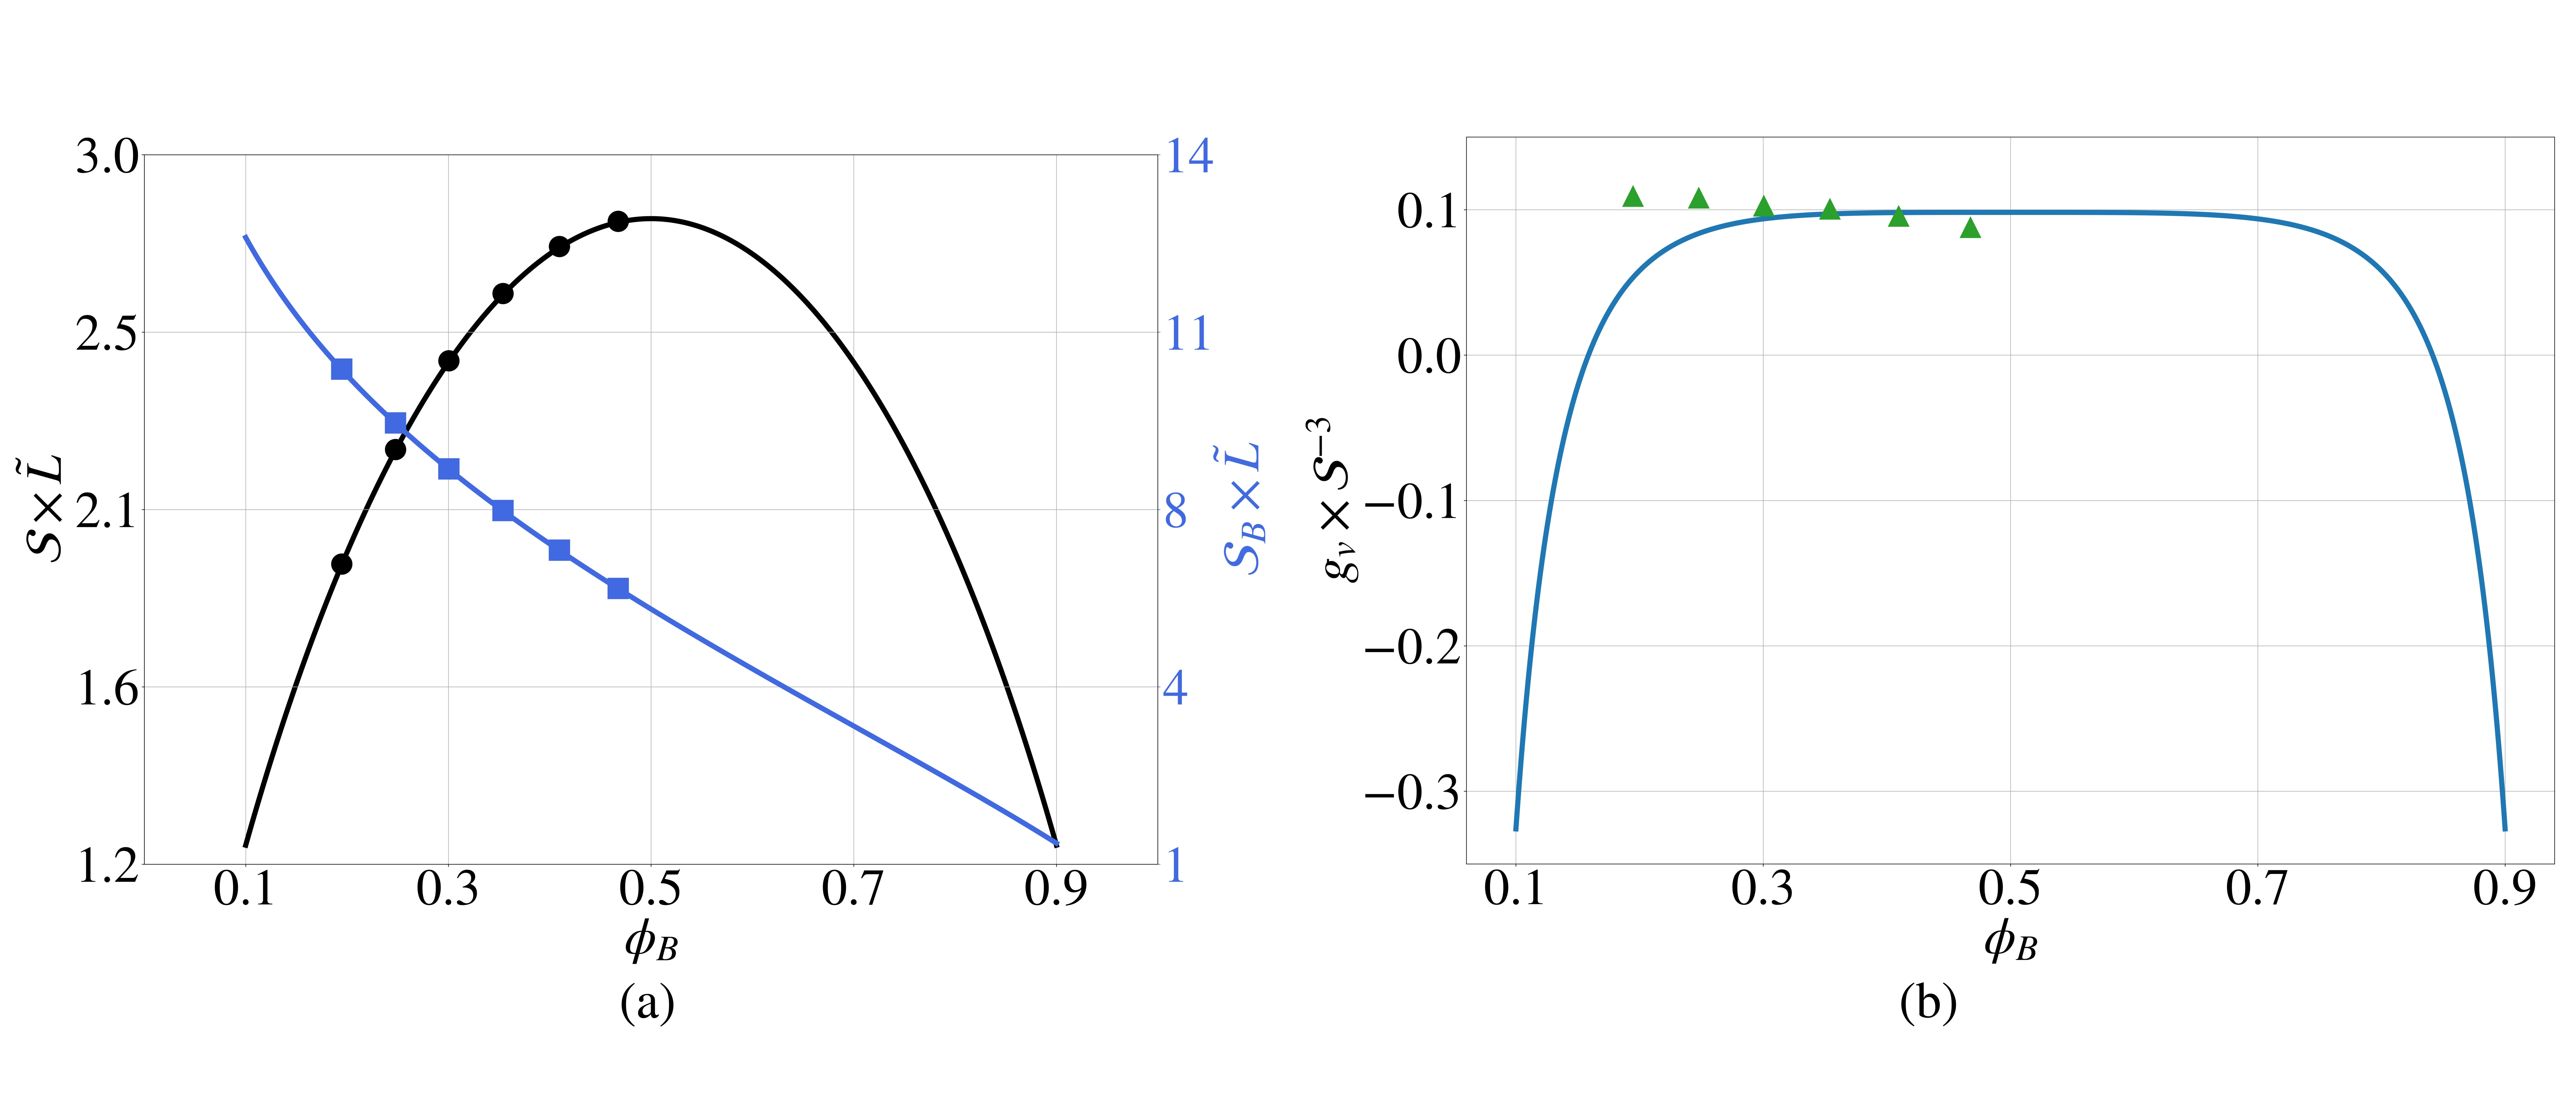
\includegraphics[width=\textwidth]{figs/Soyarslan_2Plots.jpg}
    \caption{Resultados de la comparación entre algunos resultados analíticos del modelo de Soyarslan (líneas sólidas), y las mediciones realizadas sobre espumas generados con el software (puntos): \textbf{(a)} En color negro, comparación de longitudes características reducidas, $\mathcal{S\times\hat{L}}$ es la superficie específica \eqref{eq:Soyarslan_S} multiplicada por la magnitud $\hat{L}$ definida en \eqref{eq:Soyarslan_L_hat}. La curva y puntos azules muestran la cantidad $\mathcal{S_B}$, que es la superficie específica, tomada en relación al volumen sólido. \textbf{(b)} Mediciones para la caracterización de la conectividad de la red, mediante el parámetro $g_V\times\mathcal{S}^{-3}$ \eqref{eq:Pizzagalli_g_v}, en función de la fracción sólida.}
    \label{fig:Soyarslan_2plots}
\end{figure}

\section{Rendimiento} \label{sec:4.1.3}

En la siguiente sección, se comparan las velocidades de las distintas implementaciones del código de generación de las nanoespumas. 

\subsection{Comparando las distintas versiones}
Para evaluar la eficiencia del programa, se realizaron ejecuciones de prueba sobre las 4 implementaciones distintas. 

En la fig. \ref{fig:benchmark1} puede verse el resultado de las pruebas de velocidad realizadas sobre una misma espuma de $100^3$ celdas cúbicas simples, sumando sobre 48 direcciones y con 10000 ondas. Las barras azules en la figura indican el tiempo de pared \textit{``Walltime''} medido en horas, y las barras naranjas muestran el \textit{speedup}, una métrica utilizada para medir la escalabilidad de un código computacional paralelizable, definido como

\begin{equation}
    \operatorname{speedup} = \frac{t_1}{t_N},
\end{equation}

donde $t_1$ es el tiempo requerido al correr el código en un único procesador, y $t_N$ el tiempo para $N$ procesadores. En un escenario ideal, el speedup debería tener una relación lineal con el número de procesadores utilizados. Esto significaría que cada procesador está otorgando el 100\% de su potencia computacional, lo que en la práctica representa un gran desafío \cite{Amdahl1967}.

Los resultados demuestran una clara aceleración a partir de la implementación de los cálculos mediante matrices, como era de esperarse. Llama la atención también la gran velocidad que tiene la versión implementada en GPU, incluso respecto de las versiones corridas en CPU (casi 10 veces más rápida que corriendo en 4 cores).

\begin{figure}[H]
    \centering
    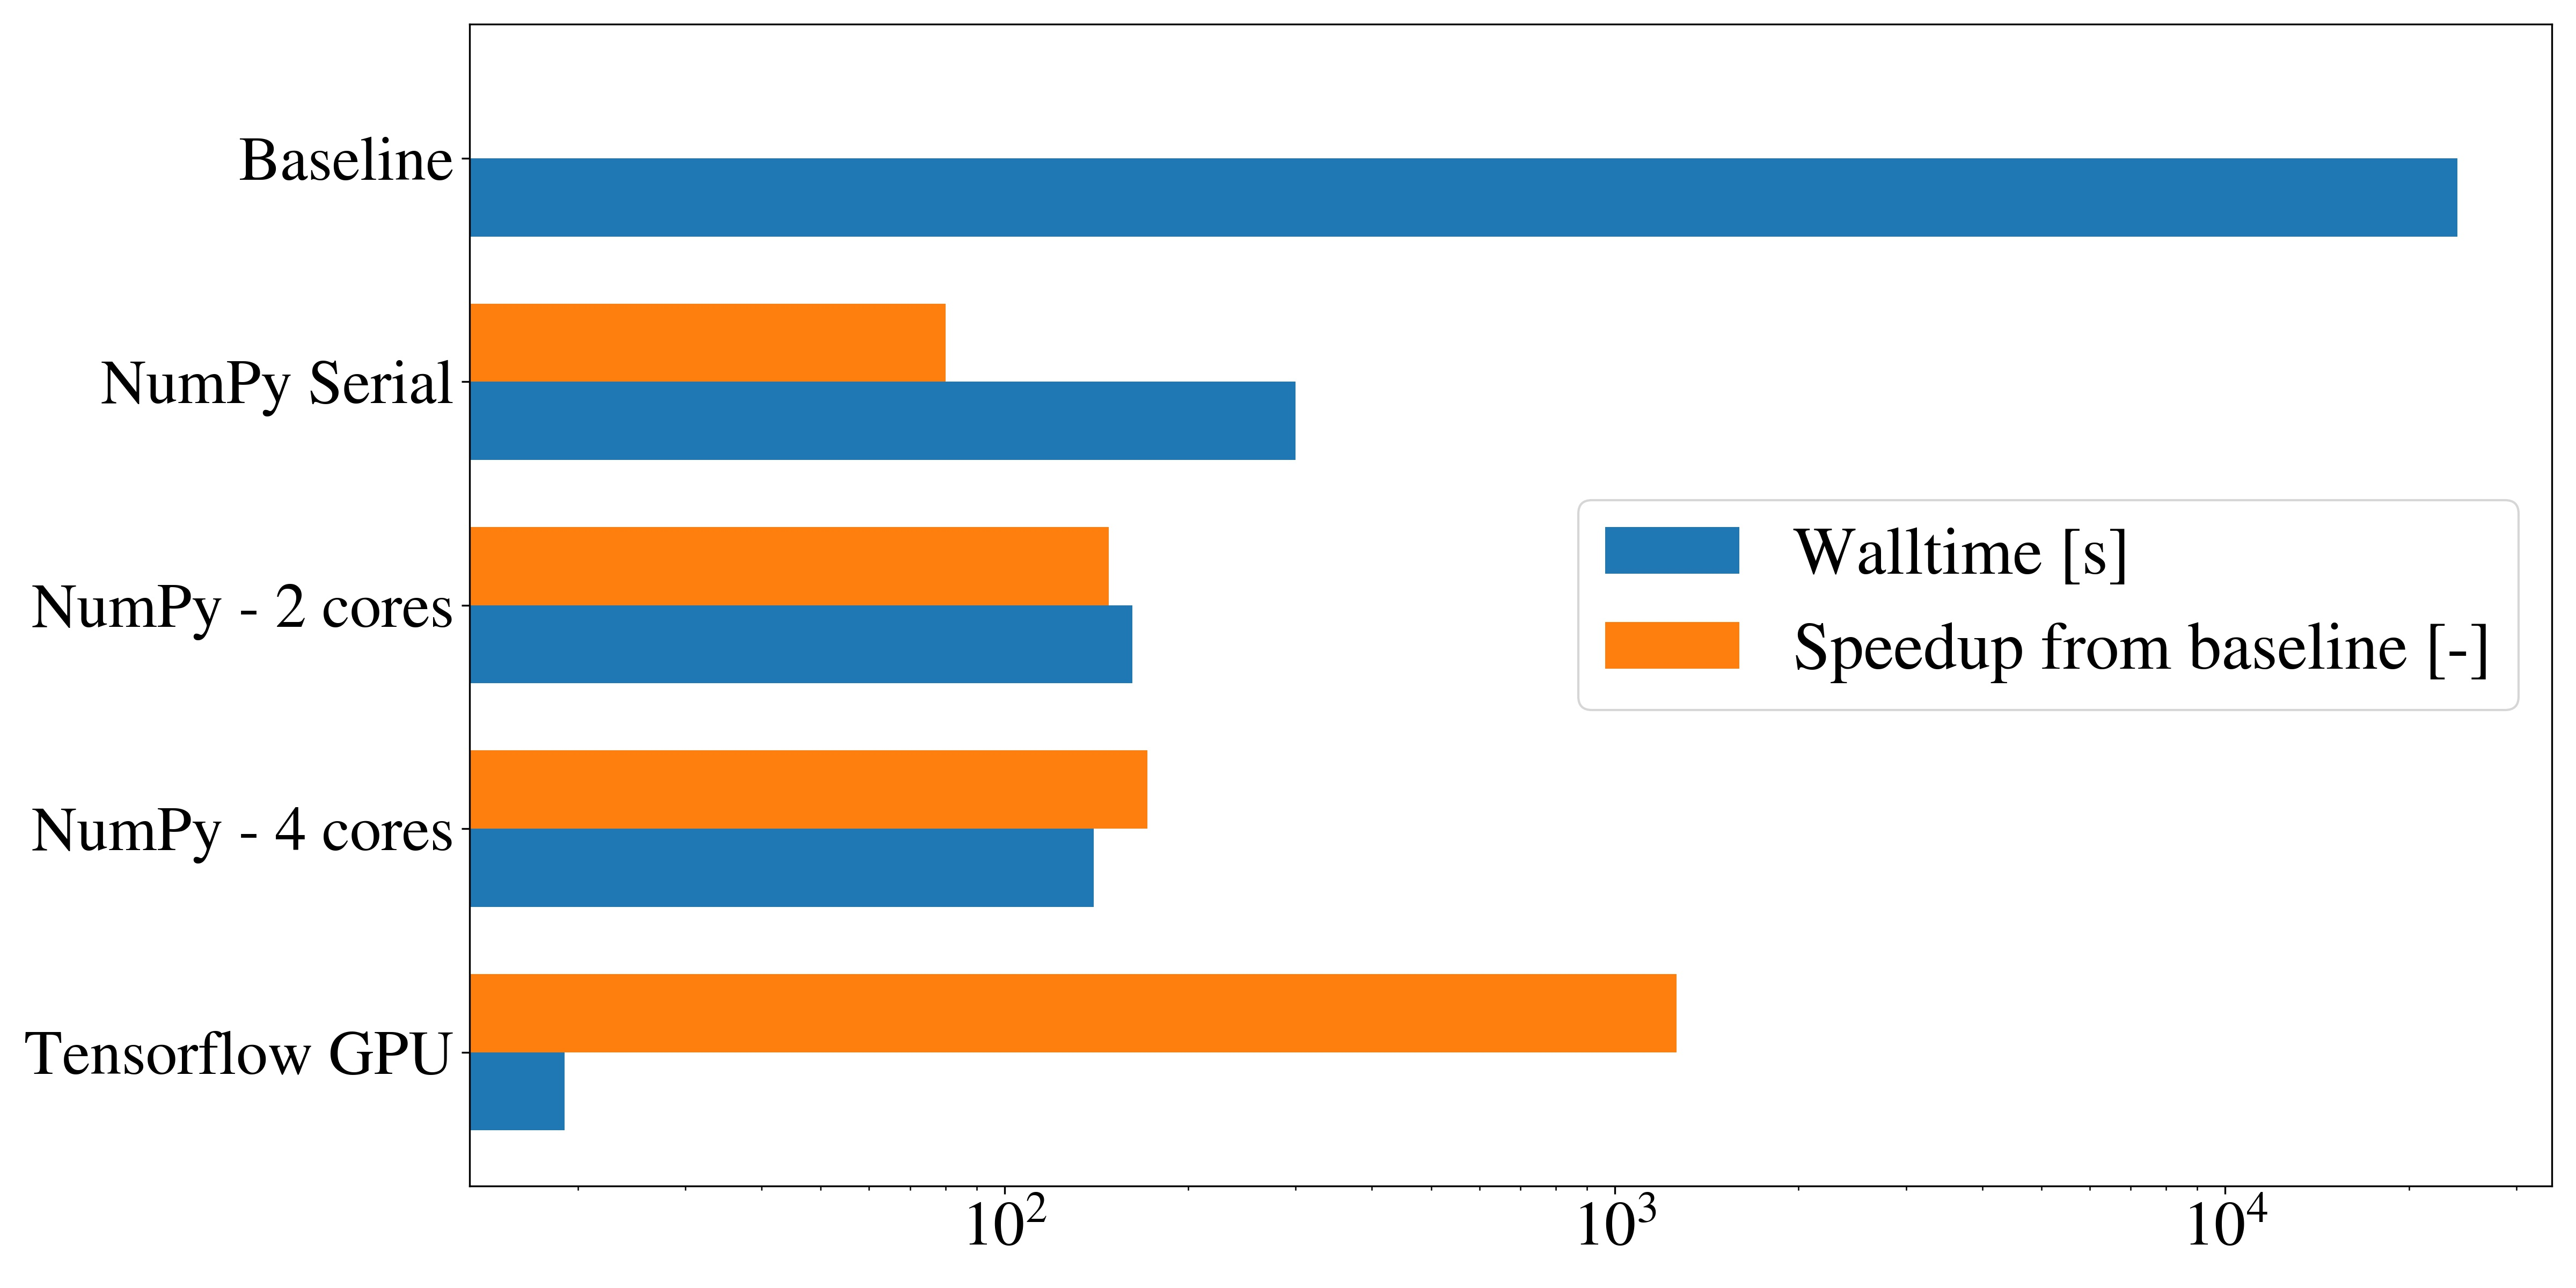
\includegraphics[width=.7\textwidth]{figs/Benchmarks1.jpg}
    \caption{Resultados en una prueba de tiempos realizada sobre las 4 versiones implementadas del código. En barras azules, el tiempo total de ejecución en segundos (Walltime); en barras naranjas , el speedup respecto del código inicial (baseline). Estas pruebas se ejecutaron en un CPU de laptop, modelo AMD Ryzen3 4000 series de 4 cores, en conjunto con una GPU NVidia K80 de 4.1 TFlops.}
    \label{fig:benchmark1}
\end{figure}

\subsection{Corrida de varios cores contra GPU}

Finalmente, para hacer un recorrido integral, resulta interesante comparar los tiempos de ejecución de las dos versiones finales del código. Para ello se realizó una ejecución en 1 y 16 cores de la versión CPU en el cluster Toko, contra una corrida en GPU de la misma espuma bcc con $300^3$ celdas unitarias y 20000 ondas. Los resultados de esta evaluación de rendimiento están comparados en la fig. \ref{fig:Benchmark2_StrScaling}.a. Nuevamente, es notorio aquí que el rendimiento de la versión GPU ha alcanzado es muy alto comparado con la versión diseñada para CPU en paralelo.

\subsection{Análisis de escala en cluster de cómputo}

La computación en paralelo, donde varios procesadores trabajan simultáneamente para generar potencia computacional y reducir el tiempo de cómputo, es una técnica usual en el desarrollo e implementación de códigos de alto desempeño. Una métrica utilizada para caracterizar cómo cambia el tiempo de cómputo al aumentar los recursos disponibles para la tarea es la \textbf{escalabilidad}. Para esta última prueba, se eligió una muestra del mismo tamaño que en la prueba anterior ($300^3$ celdas bcc cúbicas y 20000 ondas, que son alrededor de 54 millones de átomos), y se hizo una prueba de \textit{escaleo fuerte}. Es decir, fijando el tamaño de muestra, se aumenta el número de procesadores. 

Las pruebas que corresponden a este análisis se hicieron sobre los nodos del cluster Toko (\url{http://toko.uncu.edu.ar}), en particular los nodos 05,07, y mini. Los resultados de las pruebas se presentan en la fig. \ref{fig:Benchmark2_StrScaling}.b . 

\begin{figure}[H]
    \centering
    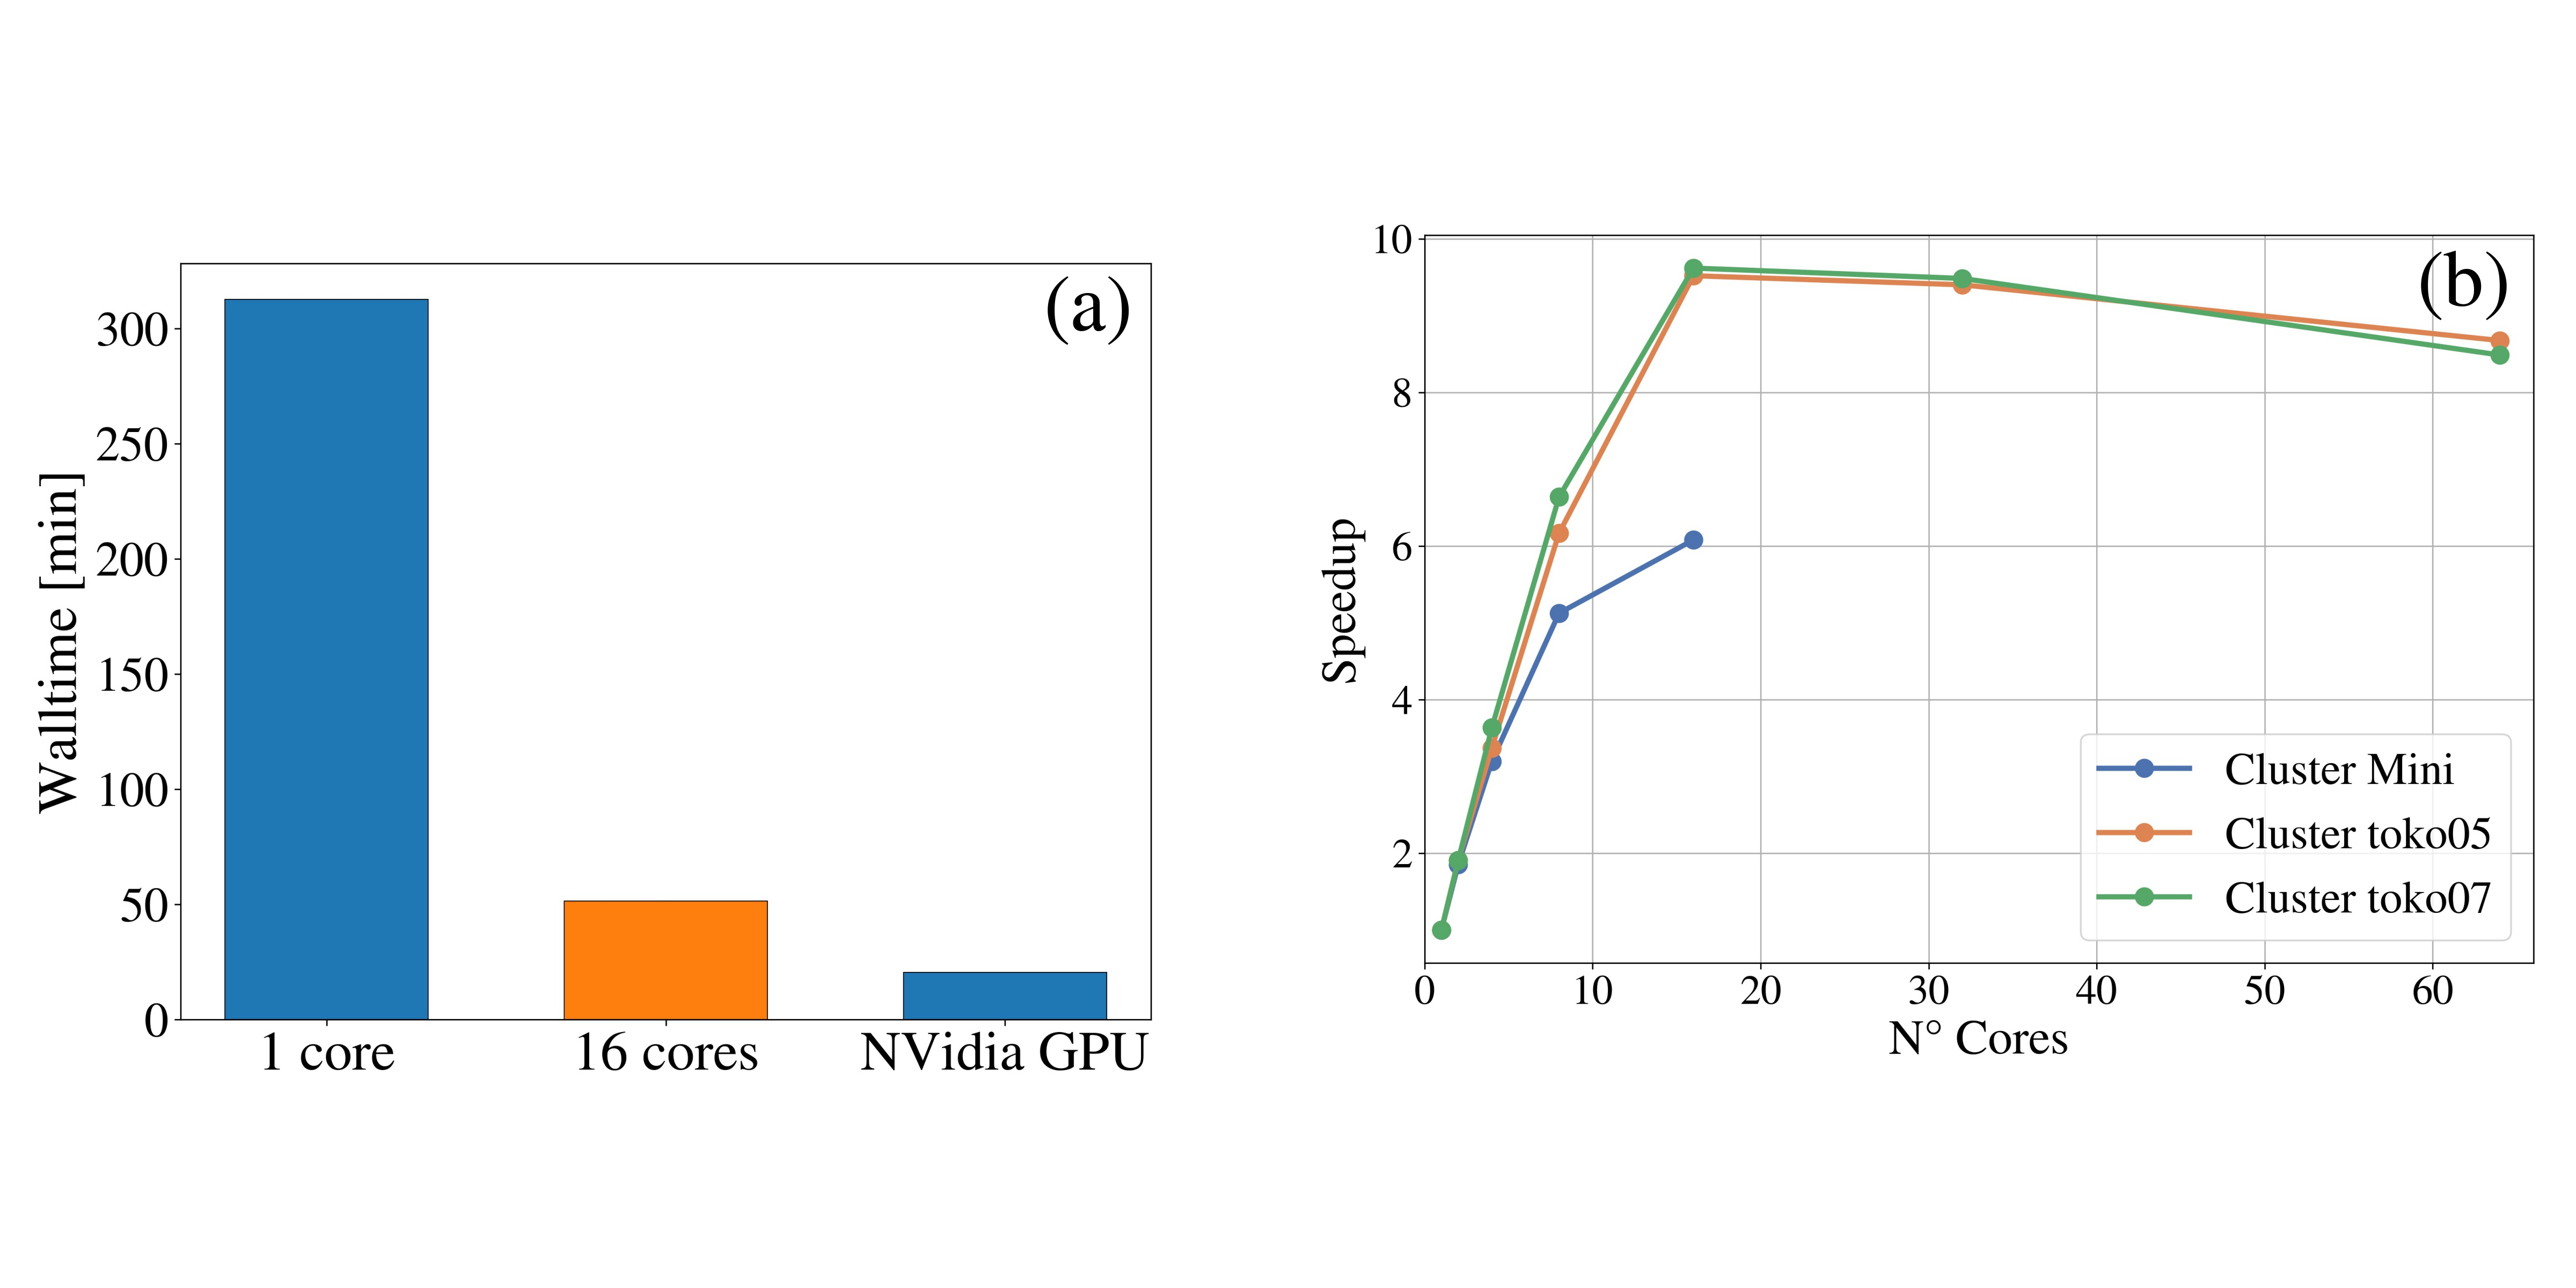
\includegraphics[width=\textwidth]{figs/Benchmark2_strScaling.jpg}
    \caption{\textbf{(a)} Comparación entre tres corridas de la misma espuma, ejecutando en serie y paralelo sobre la versión CPU, contra la versión GPU. La corrida CPU se realizó sobre uno de los nodos \textit{mini} del cluster Toko (16 cores, procesador AMD Ryzen 7, 64 Gb RAM), mientras que la ejecución GPU se realizó en Google Colab, utilizando una tarjeta NVidia K80. \textbf{(b)} Speedup vs. nro de cores para la implementación paralela del código, ejecutado sobre 3 nodos distintos del cluster Toko (FCEN-UNCuyo).}
    \label{fig:Benchmark2_StrScaling}
\end{figure}

\section{Instrucciones de uso}

\subsection{Versión script}

Esta versión del código usa la librería NumPy, en conjunto con \textit{joblib} para la división del cómputo entre los diferentes cpus. Para ejecutar, sólo se debe correr por línea de comandos algo como

\lstset{language=Bash}
\begin{lstlisting}[frame=single]
python3 build_nanofoams.py inputFile.txt 4
\end{lstlisting}

donde \textit{inputFile.txt} es un archivo de entrada que el programa necesita para la ejecución. En el mismo se insertan parámetros de entrada como las dimensiones del dominio, tamaño esperado de ligamento, densidad relativa, etc. El formato de este archivo debería ser algo similar al siguiente

\newpage

\begin{lstlisting}
###############################
# Input script nanofoams_input.txt
# Datos de entrada para el armado de las espumas
# Para usar con script build_nanofoams.py
# Nota: Las unidades de longitud son a eleccion del usuario, 
# siempre que sean consistentes en todos los parametros.
###############################

# Tipo de red cristalina (Cubica:0,BCC:1,FCC:2)
# (ante un valor distinto de 1 o 2, la red es cubica)
1

# Tamanio de caja: x_size y_size z_size (Unidad: AA)
330.3
330.3
330.3

# Parametro de red 
3.303

# Fraccion solida de la espuma
0.30

# Datos para el armado de la funcion f
# Tamanio medio de ligamento deseado 
# (este valor puede variar al generar la espuma,
# pero se le informa al usuario dicho cambio antes de continuar)
50.2
# Numero de ondas N
10000

# Constante a 
330.3

# Semilla para inicializar numeros aleatorios
42
\end{lstlisting}

El segundo parámetro que se debe ingresar por línea de comandos es el número de procesadores que se desean utilizar. \textbf{Advertencia:} Por defecto, si el usuario no ingresa ningún número, el programa inicia utilizando todos los procesadores disponibles.

\subsection{Versión notebook}

El cuaderno que fue preparado para este trabajo está explicado en modo autocontenido en el notebook, referirse allí para instrucciones de uso.

\printbibliography
\end{document}


